\begin{figure*}
  \centering
    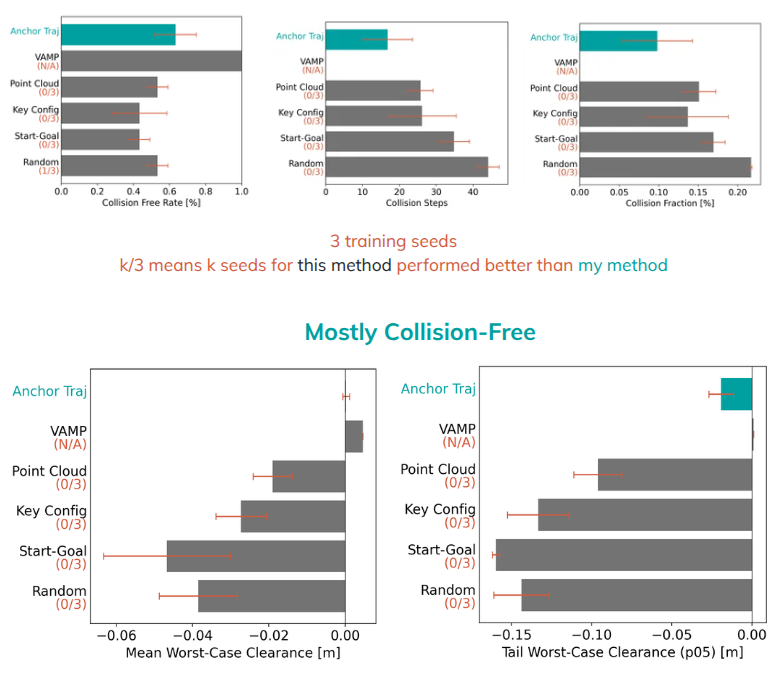
\includegraphics[width=\textwidth]{figs/eval.png}
  \caption{Collision-avoidance evaluation across three training seeds. Anchor Traj denotes the proposed diagnostic anchor conditioning method. VAMP is shown as an oracle-like upper bound rather than a learned conditioning baseline. Point Cloud uses a PointNet++ environment encoder, Key Config uses PRESTO key configurations, Start-Goal does not condition on environment information, and Random uses random environment codes. Anchor Traj achieves the strongest learned-model performance across collision-free rate, collision steps, collision fraction, and worst-case clearance metrics.}\label{fig:eval}
\end{figure*}